\documentclass[10pt,conference]{IEEEtran}
\IEEEoverridecommandlockouts
\usepackage[T1]{fontenc}
\usepackage[utf8]{inputenc}
\usepackage{amsmath,amssymb,booktabs,graphicx,tabularx}
\usepackage{microtype}
\usepackage{cite}
\usepackage[hidelinks]{hyperref}
\usepackage{balance}
\newcommand{\eps}{\varepsilon}
\newcommand{\R}{\mathcal{R}}
\newcommand{\I}{\mathbf{1}}
\newcommand{\D}{\mathcal{D}}
\title{Beyond Accuracy: Auditing Predictive and Explanatory Multiplicity in Neural Intrusion Detection}
\author{\IEEEauthorblockN{Silja Kluge}\IEEEauthorblockA{CortAIx Labs, Thales Deutschland, Ditzingen, Germany\\Eberhard Karls University of T\"ubingen, T\"ubingen, Germany\\silja.kluge@thalesgroup.com}}
\begin{document}
\maketitle
\begin{abstract}
Intrusion detectors are frequently selected using aggregate predictive scores, although similarly scoring models need not agree on individual security events or on the features explaining their decisions. We audit predictive and explanatory multiplicity in binary network intrusion detection using 630 multilayer perceptrons (63 candidates in each of ten training origins) evaluated on the fixed NSL-KDD test partition. Within the complete candidate collections, mean pairwise prediction disagreement is 3.80\%, while 15.81\% of test instances receive conflicting labels. Restricting the collections to models within 0.1 percentage points of the best validation accuracy retains 34.3 models per origin on average and still yields 3.70\% disagreement. Crucially, 2,176 attack instances (16.96\% of attacks) are unanimously classified as benign by every candidate in every origin. The global SHAP-importance vectors overlap substantially, but local attribution variance is larger on contested than unanimous predictions (0.0191 versus 0.0089, nine origins with complete local tables). These observations separate three audit targets: model-dependent alerts, model-dependent explanations, and stable but incorrect decisions. We discuss their implications for uncertainty-aware cyber-defense evaluation, without treating model consensus as a calibrated reliability guarantee.
\end{abstract}
\begin{IEEEkeywords}
Intrusion detection, predictive multiplicity, Rashomon set, SHAP, explanation stability, cyber defense
\end{IEEEkeywords}
\section{Introduction}
Machine-learning intrusion detection can inform alert generation, incident triage, and automated defensive responses. In security-sensitive environments, including military and mission-critical networks, decisions made from such alerts may affect operational continuity and investigative workload. Accuracy and F1 score remain essential evaluation measures, but they do not answer whether the decision for a particular network event would change if another similarly accurate model were deployed.

This question is related to the Rashomon effect: a learning task may admit many well-performing predictors, rather than one uniquely supported decision rule \cite{breiman2001,black2022,hsu2022}. Predictive multiplicity is operationally relevant when two plausible intrusion detectors assign different labels to the same event. Explanation multiplicity creates a separate difficulty: even when the predicted label is the same, the feature attribution used to justify an alert can depend on the chosen model \cite{brunet2022,laberge2023}. An assessment restricted to a single fitted detector conceals both sources of variation.

For cyber defense, a further distinction is important. Disagreement can identify events for which the model choice matters, but it cannot identify an event that all considered models miss. We therefore examine not only unstable decisions and explanations, but also \emph{persistent unanimous errors}, defined as mistakes shared by all candidates across repeated training origins. We do not assume that disagreement is a calibrated probability of attack or that consensus establishes correctness.

We address three research questions: \textbf{RQ1}: How much predictive disagreement persists among validation-selected, similarly performing intrusion detectors? \textbf{RQ2}: How is predictive disagreement related to global and local SHAP attribution variability? \textbf{RQ3}: Which security-relevant errors remain undetected by a disagreement-only audit, and how are they distributed across attack families?

Our contributions are (i) a replication-aware empirical audit of 630 neural intrusion detectors across ten training origins; (ii) a sensitivity study that distinguishes nearly all-inclusive from genuinely selective Rashomon thresholds; (iii) a cross-model comparison of global explanations and local SHAP instability, explicitly separating analyses with ten and nine available origins; and (iv) a security-oriented distinction between contested detections and attacks missed unanimously by the entire empirical model collection.

\section{Background and Related Work}
\subsection{Predictive Multiplicity and Rashomon Sets}
The Rashomon effect describes the presence of alternative models with comparably strong performance \cite{breiman2001}. Black \emph{et al.} distinguish diversity in model construction from diversity in individual predictions \cite{black2022}. Marx \emph{et al.} formalize predictive multiplicity using ambiguity and discrepancy, demonstrating that models close in aggregate loss may differ at specific instances \cite{marx2020}. Hsu and Calmon analyze the capacity of a set of good models to support diverse classifications \cite{hsu2022}.

A finite study can observe only an \emph{empirical} Rashomon set: models trained under the specified candidate-generation process that satisfy a performance criterion. Its size does not estimate the number of all possible near-optimal classifiers. In particular, a large candidate collection is not evidence of strong performance-based selection if the chosen tolerance admits essentially every trained model. We report the selected model count alongside the resulting disagreement, and investigate more restrictive tolerances.

\subsection{Explanations and Security Interpretation}
SHapley Additive exPlanations (SHAP) decomposes a model output into a baseline and feature-specific contributions, based on Shapley values \cite{shapley1953,lundberg2017}. A SHAP explanation applies to the explained model and output; it need not describe another equally plausible classifier. Brunet \emph{et al.} identify limitations of taking one model's explanations as unique when multiple models are plausible \cite{brunet2022}, while Laberge \emph{et al.} investigate partial consensus of feature attributions across Rashomon sets \cite{laberge2023}. Thus, prediction consensus and attribution consensus should be measured separately.

Explainability has also been studied in network intrusion detection, for example through hybrid oracle--explainer approaches \cite{szczepanski2020} and broader cybersecurity XAI surveys \cite{zhang2022}. A recent IDS reliability audit by Maseno \emph{et al.} compares SHAP attributions with permutation importance, retraining stability, and spurious-feature probes across model families \cite{maseno2026}. That work investigates whether explanations are faithful and robust; our narrower analysis instead measures variation \emph{across comparably accurate candidate models} and links it to an explicitly security-oriented consensus audit. Recent work on resolving predictive multiplicity also considers ways to reconcile disagreeing models \cite{haghighat2026}. We do not propose a reconciliation algorithm or claim that disagreement can be removed without changing the model family. Adversarial evasion studies highlight that behavior beyond a mean score matters for detection effectiveness \cite{pawlicki2020}, but our study is not an adversarial robustness evaluation: we quantify sensitivity to plausible \emph{model selection} under a fixed test distribution, not robustness to adaptive attackers or deployment drift.

\section{Methodology}
\subsection{Candidate Generation and Validation Selection}
For origin $o$, let $\mathcal F_o$ be the finite set of trained classifiers, and let $A_o^{\mathrm{val}}(f)$ denote validation accuracy. We construct the empirical Rashomon set
\begin{equation}
\R_o(\eps)=\{f\in\mathcal F_o:A_o^{\mathrm{val}}(f)\geq \max_{g\in\mathcal F_o} A_o^{\mathrm{val}}(g)-\eps\}.
\label{eq:rashomon}
\end{equation}
Here $\eps$ is an \emph{absolute} accuracy difference; $\eps=0.001$ means 0.1 percentage points. Sets are selected independently in each origin, with validation data only. The held-out test set is never used to choose models. Because the original analysis stores complete-candidate predictions and class-specific explanations, model-pair statistics can be filtered by membership in a subsequently reconstructed $\R_o(\eps)$ without retraining. We distinguish such reconstructions from new attribution computations.

\subsection{Predictive Multiplicity}
For test set $T$ of size $N$, predicted label $\hat y_f(x)$, and $f\neq g$, the disagreement rate is
\begin{equation}
 D_o(f,g)=\frac{1}{N}\sum_{x\in T}\I[\hat y_f(x)\neq\hat y_g(x)].
 \label{eq:pair}
\end{equation}
Mean pairwise disagreement averages $D_o$ over unordered pairs within the selected set. Sample ambiguity records whether any models disagree,
\begin{equation}
 \mathrm{Amb}_o=\frac{1}{N}\sum_{x\in T}\I[|\{\hat y_f(x):f\in\R_o\}|>1],
 \label{eq:ambiguity}
\end{equation}
and the pointwise conflict ratio is
\begin{equation}
 c_o(x)=1-\frac{\max_y\sum_{f\in\R_o}\I[\hat y_f(x)=y]}{|\R_o|}.
 \label{eq:conflict}
\end{equation}
Unlike ambiguity, $c_o(x)$ distinguishes a narrowly split committee from a nearly unanimous one. It measures vote disagreement, not an attack probability.

\subsection{Global and Local Explanation Multiplicity}
For a model $f$, explained test instance $x$, output class $c$, and feature $j$, let $\phi_{f,c,j}(x)$ be its SHAP attribution. All models within an origin use the same background points and the same explained test instances. Global feature importance is $I_{f,c,j}=|E|^{-1}\sum_{x\in E}|\phi_{f,c,j}(x)|$. The implementation retains the 50 highest-ranked features per model and class; we compare these \emph{truncated} vectors by cosine distance and compare top-20 feature sets by Jaccard similarity. Missing entries in a stored top-50 vector are assigned zero for the pairwise calculation. Accordingly, global cosine distance does not quantify full-dimensional local explanation disagreement.

The stored local tables instead permit a samplewise cross-model variance audit. For a complete $|\R_o|=63$ collection, let
\begin{equation}
 V_o(x)=\frac{1}{Cd}\sum_{c=1}^{C}\sum_{j=1}^{d}
 \mathrm{Var}_{f\in\R_o}(\phi_{f,c,j}(x)),
 \label{eq:local}
\end{equation}
where $C=2$ model outputs and $d$ is the encoded feature count. The variance uses the implementation's stored per-feature values. We also inspect cross-model attribution sign instability $\min(p_+,1-p_+)$, where $p_+$ is the fraction of positive attributions. These statistics are averaged first over feature/class groups within an instance, then over explained instances within an origin. Local explanation findings are descriptive and cannot be interpreted as causal explanations.

\subsection{Interpretation of the Audit Levels}
The three research questions deliberately operate at different granularities. Pairwise disagreement measures the average fraction of changed decisions between two models, whereas ambiguity asks whether \emph{any} model choice changes the event label. Both are properties of the empirical candidate pool, not of an individual detector in isolation. Local attribution variance conditions on a fixed event and measures disagreement over fitted models, whereas a global feature-ranking measure first aggregates across events. Finally, a persistent consensus error requires external ground truth: it cannot be diagnosed from model votes alone. These distinct levels preclude a single score that simultaneously represents classification quality, uncertainty, and explanation reliability. We therefore report them separately and avoid combining them into a composite confidence measure.

\subsection{Security-Oriented Consensus Audit}
For each test event, we distinguish \emph{unanimous normal}, \emph{contested}, and \emph{unanimous attack} outcomes. Combining these categories with ground-truth labels yields operationally distinct errors: a unanimous false negative is a malicious event that every candidate classifies as benign; a contested event has at least one pair of different predictions. A \emph{persistent} unanimous false negative is missed by all candidates in \emph{all ten} origins; a \emph{persistent} conflict is contested in every origin. The two persistent definitions are mutually exclusive. To interpret failure modes, we use the original NSL-KDD attack-family labels (DoS, Probe, R2L, U2R) for the fixed test records.

\subsection{Aggregation and Replication}
Each origin uses its own training/validation split and disjoint training-seed namespace, but all origins share the same 22,544 test observations. We compute statistics within origins and report mean $\pm$ sample standard deviation over origins, not over model pairs. Pairs share component models; thus 1,953 pairs per origin are not independent replicates. For the local variance reanalysis, complete sample-feature tables were available for origins 1--9; origin 10 had a summary but no downloadable \texttt{shap\_variability.csv}. We therefore use $n=9$ for the new per-instance comparisons and $n=10$ for other results. The same 128 explained test observations are reused across origins, so origin-level variation does not represent uncertainty over independently resampled test sets.

\section{Experimental Setup}
\subsection{Dataset and Preprocessing}
We use NSL-KDD \cite{tavallaee2009}, mapping all attack labels to the positive class and \texttt{normal} to the negative class. Each origin splits the predefined \texttt{KDDTrain+} partition into 80\% training and 20\% stratified validation examples (100,778 and 25,195 observations). The same predefined \texttt{KDDTest+} partition of 22,544 observations, including 12,833 attacks and 9,711 normal records, remains held out. Labels and the benchmark difficulty column are excluded as predictors. Numerical fields are median-imputed and standardized; categorical fields (protocol, service, and connection flag) are mode-imputed and one-hot encoded. All preprocessing is fitted on the training subset of each origin and applied unchanged to its validation and test data.

\subsection{Model Pool and Attribution Protocol}
Ten origins each contain 63 multilayer perceptrons (MLPs): one reference, 20 seed variants, 20 bootstrap-resampled variants, 20 architecture/activation variants, and two stratified-subset variants using 75\% and 50\% of the origin training examples. The reference network uses hidden widths $(128,64)$, ReLU activations, batch normalization, and dropout $0.2$. Architecture variants use seven width choices from $(32,16)$ to $(256,128)$ crossed with ReLU, tanh, and leaky ReLU, excluding the reference combination. Candidate blocks were separately constructed and should not be read as independent controlled interventions.

Models were optimized using AdamW (learning rate $10^{-3}$, weight decay $10^{-4}$, batch size 256), cross-entropy loss, and validation-loss early stopping with patience five, for at most 20 epochs. Predictive measures are accuracy, macro-F1 and log loss. For explanations, \texttt{shap.DeepExplainer} uses 64 training-background examples and 128 fixed test examples (50 normal, 78 attack), with identical selected indices across origins. We examine $\eps\in\{0.0005,0.001,0.005,0.010\}$; the prior stored full-set analysis was originally generated with $\eps=0.015$.

\subsection{Available Artifacts and Reanalysis Protocol}
The ten stored origin folders contain model validation/test metrics, model identifiers, pairwise prediction-disagreement tables, and pairwise global-explanation comparisons. Reconstructing a stricter Rashomon set consists of selecting candidate IDs from the validation-accuracy table and retaining only pairs whose endpoints belong to that set. This does not change fitted weights, prediction scores, attribution baselines, or the fixed test set. It avoids the inappropriate use of test accuracy for model selection, but it also means that explanations under stricter thresholds are \emph{filtered} rather than independently recomputed.

For a complementary sample-level security audit, we join per-origin sample-disagreement summaries across origins using their fixed test indices and original attack labels. The three consensus outcomes are mutually exclusive within each origin. Persistent categories are obtained by intersecting the per-origin outcomes over all ten seeds. For the local explanation reanalysis we aggregate stored feature/class-specific variance and sign-instability by test index, merge each with the corresponding full-pool pointwise conflict ratio, and then compare contested versus unanimous instances \emph{within each origin}. Originwise statistics are averaged only at the final stage. We do not treat 128 explained test instances as independently sampled anew in each origin, nor do we perform significance tests on the hundreds of thousands of dependent model pairs.

\section{Results}
\subsection{Performance and Selection Sensitivity}
Across the 630 models, mean held-out accuracy is $0.7869$ and mean macro-F1 is $0.7867$. Mean validation accuracy is $0.9959$, a 20.9-percentage-point gap to held-out accuracy (Fig.~\ref{fig:gap}). This is a major generalization concern. While NSL-KDD has a structurally distinct official test partition, the present evidence does not isolate whether the gap arises from distribution shift, overfitting, or pipeline-specific effects; we therefore do not attribute it uniquely.

At $\eps=0.010$ every candidate is selected. At $\eps=0.005$ exactly one candidate is excluded across the ten origins. By contrast, $\eps=0.001$ retains $34.3\pm6.2$ models per origin, and $\eps=0.0005$ retains $11.7\pm4.8$. Selection substantially changes the model population but does not eliminate disagreements (Table~\ref{tab:threshold}; Fig.~\ref{fig:select}). Thus our complete-set findings are an audit of the generated model pool, while the narrower-threshold pair results demonstrate persistence under nontrivial performance filtering.

\begin{figure}[t]
\centering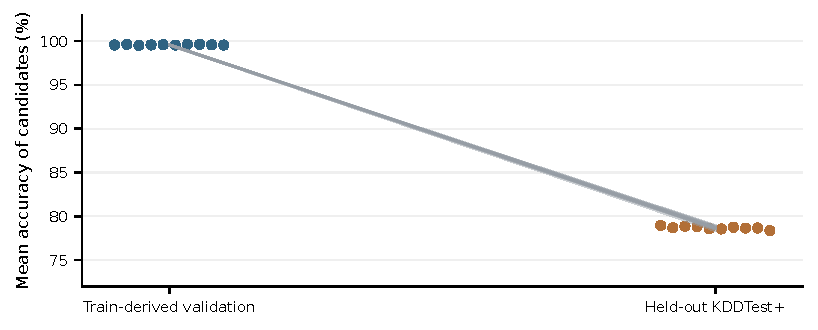
\includegraphics[width=\columnwidth]{validation_test_gap.pdf}
\caption{Mean candidate accuracy in each origin on train-derived validation and held-out \texttt{KDDTest+}. Lines connect the same ten origins, not independent test partitions.}
\label{fig:gap}
\end{figure}

\begin{table}[t]
\caption{Validation tolerance, selected models, predictive disagreement and global explanation divergence. Origin-level means ($n=10$).}
\label{tab:threshold}\centering
\setlength{\tabcolsep}{4pt}
\begin{tabular}{@{}rrrr@{}}\toprule
$\eps$ & Models/origin & Disagree. (\%) & SHAP cosine \\ \midrule
0.0005 & 11.7 & 3.590 & 0.0468 \\
0.0010 & 34.3 & 3.697 & 0.0510 \\
0.0050 & 62.9 & 3.800 & 0.0593 \\
0.0100 & 63.0 & 3.801 & 0.0594 \\
\bottomrule\end{tabular}
\end{table}

\begin{figure}[t]
\centering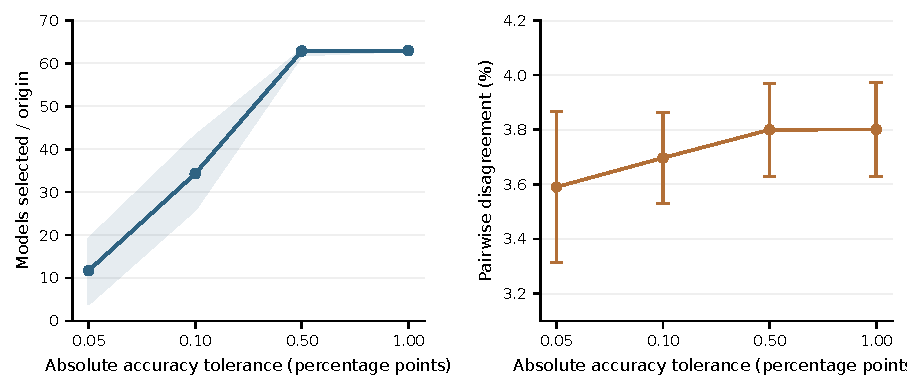
\includegraphics[width=\columnwidth]{rashomon_selection.pdf}
\caption{Selection size and pairwise disagreement across increasingly permissive validation-accuracy tolerances. Shading gives the minimum--maximum origin range; right-hand error bars show one sample standard deviation.}
\label{fig:select}
\end{figure}

\subsection{Predictive Multiplicity and Persistent Conflict}
For the complete 63-model sets, mean pairwise disagreement is $3.801\pm0.171\%$, whereas within-origin sample ambiguity is $15.811\pm1.326\%$. The largest pairwise disagreement within an origin averages $7.53\pm0.86\%$. These measures differ because a test event can be contested by some models even when most model pairs agree. At $\eps=0.001$, pairwise disagreement remains $3.697\pm0.166\%$, despite the much smaller selected sets.

Disagreement concentrates on particular samples rather than being uniformly distributed. Across the fixed 22,544 test samples, 17,766 (78.8\%) are never contested in any origin, whereas 2,275 (10.1\%) are contested in \emph{all} ten origins (Fig.~\ref{fig:persistence}). Among the always-contested instances, 1,679 are attacks and 596 are normal records. This persistence identifies a subset of test cases particularly sensitive to model selection but does not show that such cases are necessarily novel attacks or intrinsically adversarial.

\begin{figure}[t]
\centering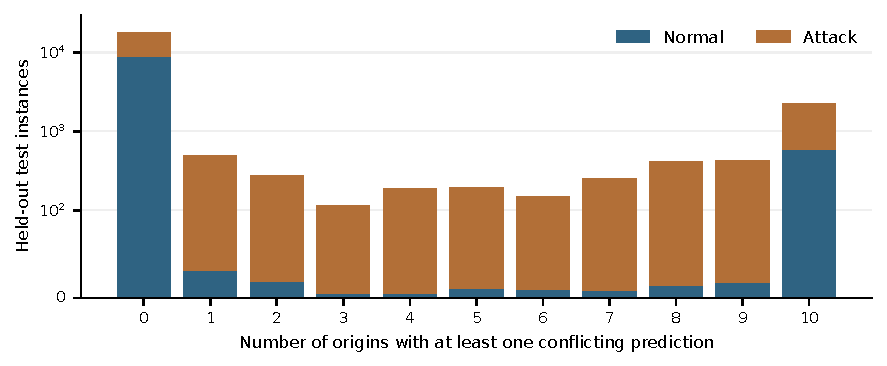
\includegraphics[width=\columnwidth]{conflict_persistence.pdf}
\caption{How often each fixed test event is contested across the ten complete model collections, split by true label. The vertical axis is symmetric-log to display the tail.}
\label{fig:persistence}
\end{figure}

\subsection{Security Failure Modes: Contested Versus Unanimous}
The confusion-oriented consensus audit reveals a distinct limitation of using disagreement alone for security triage (Fig.~\ref{fig:consensus}). Within an origin, on average $2,955\pm173$ attack instances are unanimously predicted normal; another $2,915\pm299$ attack instances are contested. Unanimously predicted-normal events therefore include a mean 24.9\% malicious cases, despite their absence of within-committee conflict. Conversely, contested events are 81.6\% attack-labeled in this \emph{particular} attack-enriched benchmark. These conditional proportions are \emph{not} deployment probabilities and would change under realistic base rates.

Across \emph{all} ten origins, 2,176 of 12,833 attacks (16.96\%) are persistently and unanimously labeled benign. A triage policy based solely on committee disagreement would not flag these incidents, even if it flagged every contested event. By family, persistent unanimous misses are most pronounced for remote-to-local (R2L) events: 1,690 of 2,885 (58.58\%) are missed by every tested model in every origin. The corresponding rates are 5.36\% for DoS (400/7,460), 3.02\% for Probe (73/2,421), and 19.40\% for user-to-root (U2R; 13/67). For comparison, persistent conflict occurs on 9.02\% of DoS, 23.92\% of Probe, 13.41\% of R2L, and 59.70\% of U2R records (Fig.~\ref{fig:families}). U2R has only 67 examples, so percentages should not be overinterpreted.

\begin{table}[t]
\caption{Persistent unanimous misses and conflicts across ten origins by NSL-KDD attack family. Counts are based on the fixed test set; the two outcomes are mutually exclusive.}
\label{tab:families}\centering
\setlength{\tabcolsep}{4pt}
\begin{tabular}{@{}lrrrr@{}}\toprule
Family & Test $n$ & Missed $n$ & Missed (\%) & Conflict (\%) \\ \midrule
DoS & 7,460 & 400 & 5.36 & 9.02 \\
Probe & 2,421 & 73 & 3.02 & 23.92 \\
R2L & 2,885 & 1,690 & 58.58 & 13.41 \\
U2R & 67 & 13 & 19.40 & 59.70 \\ \midrule
Total attacks & 12,833 & 2,176 & 16.96 & 13.08 \\
\bottomrule\end{tabular}
\end{table}

The persistent failure modes vary sharply at the attack-subtype level. Five subtypes account for most of the unanimous misses: \texttt{guess\_passwd} (779/1,231), \texttt{warezmaster} (353/944), \texttt{snmpguess} (326/331), \texttt{mailbomb} (278/293), and \texttt{snmpgetattack} (171/178). These counts are not simply hard cases on which alternative classifiers disagree: they are examples on which the entire observed candidate pool returns the same wrong benign label. A disagreement-only evaluation would characterize their decisions as stable while missing the underlying detection failure.

\begin{figure}[t]
\centering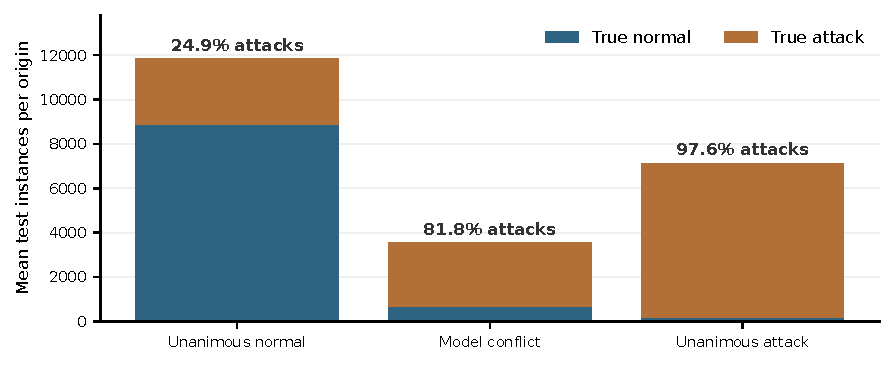
\includegraphics[width=\columnwidth]{security_consensus.pdf}
\caption{Mean test-set counts per origin by model-consensus outcome and true label. Numbers above bars report the attack-labeled share within each outcome group, not calibrated attack risks.}
\label{fig:consensus}
\end{figure}

\begin{figure}[t]
\centering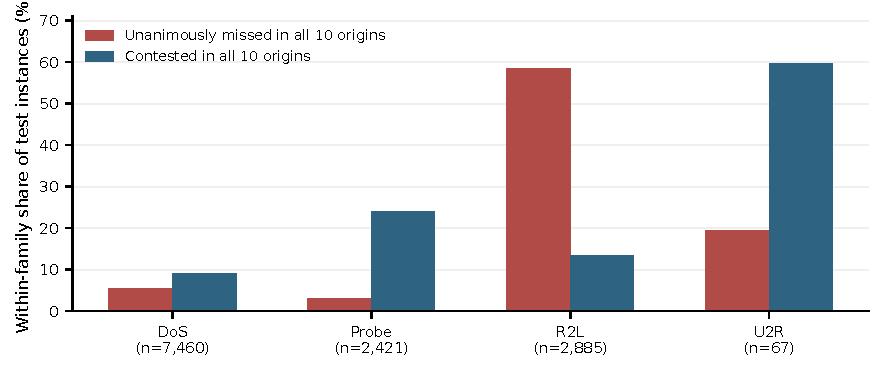
\includegraphics[width=\columnwidth]{attack_families.pdf}
\caption{Two mutually exclusive persistent failure modes by NSL-KDD attack family: unanimous false negative versus within-origin disagreement, each in all ten origins.}
\label{fig:families}
\end{figure}

These observations support a security-specific distinction between \emph{uncertain decisions} and \emph{consistently wrong decisions}. The first can, in principle, be surfaced by committee disagreement. The second requires other evidence, such as independent detection mechanisms, contextual telemetry, or post-hoc error analysis. Agreement alone should not be treated as a proxy for high confidence.

\subsection{Global Explanatory Multiplicity}
The classwise top-50-truncated SHAP importance vectors have mean pairwise cosine distance $0.0594\pm0.0031$; top-20 feature-set Jaccard similarity is $0.781\pm0.026$ across ten origins. The leading attack-class features predominantly involve destination-host and service-level traffic statistics, including \texttt{dst\_host\_srv\_count}, \texttt{dst\_host\_same\_srv\_rate}, \texttt{dst\_host\_rerror\_rate}, and flag \texttt{S0}. Thus, models tend to agree on broad importance themes but do not produce identical attribution rankings or magnitudes.

Matching predictive model pairs to their two classwise explanation comparisons, the mean within-origin Spearman correlation between pairwise prediction disagreement and global SHAP cosine distance is $\rho=0.175\pm0.071$ ($n=10$). The association is positive but modest: different labels do not generally imply proportionally different \emph{global} rankings, and global agreement does not prove stable explanations for an individual detection. No pair-level inferential test is justified because model pairs overlap.

\subsection{Local Explanatory Multiplicity}
A new instance-level analysis of the nine complete local SHAP tables characterizes cross-model attribution variance on the same 128 test instances in every origin. Within an origin, $18.7\pm2.8$ of these instances are contested, leaving $109.3\pm2.8$ unanimously labeled. Mean samplewise cross-model attribution variance is $0.0191\pm0.0023$ for contested instances versus $0.0089\pm0.0009$ for unanimous instances (Fig.~\ref{fig:local}). The mean originwise Spearman association between pointwise conflict ratio and mean local SHAP variance is $\rho=0.444\pm0.046$.

Class composition partly affects these unstratified means: only about three of the 50 normal examples per origin are contested, compared with about 16 of the 78 attack examples. Restricting comparisons to attack-labeled examples, the corresponding means are $0.0176$ (contested) and $0.0107$ (unanimous), with mean within-origin $\rho=0.383$. The positive descriptive association therefore persists within the attack class. Importantly, unanimous decisions do not have zero attribution variance; the SHAP explanation can depend on the selected model even when its label does not. Average sign-instability scores are $0.063$ on unanimous and $0.068$ on contested examples; this modest contrast should not be confused with the much larger variance difference.

\begin{figure}[t]
\centering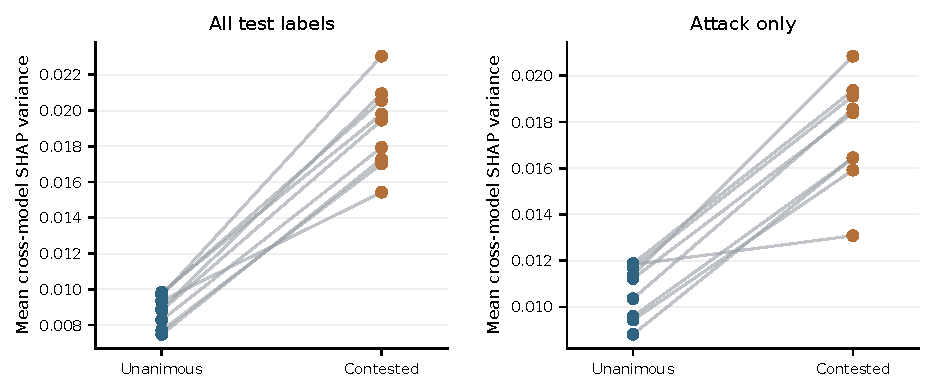
\includegraphics[width=\columnwidth]{local_shap_conflict.pdf}
\caption{Per-origin mean SHAP attribution variance on unanimous versus contested explained instances ($n=9$ complete local tables). Each line links the two groups within one origin; right: attack-labeled subset only.}
\label{fig:local}
\end{figure}

The local analysis and the global pairwise correlation address different statistical levels: $V_o(x)$ compares attribution variability across models \emph{for one event}; global cosine distance compares classwise aggregated feature-importance vectors \emph{between two models}. They should not be pooled into one correlation or used interchangeably.

\subsection{Answering the Research Questions}
\textbf{RQ1:} Validation accuracy alone does not uniquely determine per-event decisions. The all-inclusive model pools yield 3.80\% pairwise disagreement and 15.81\% ambiguity, and disagreement persists at 3.70\% even when the Rashomon criterion filters out nearly half the models on average. \textbf{RQ2:} Global feature importances are similar, yet they are not identical; more importantly, local attribution variance is higher on contested events and remains nonzero on unanimous ones. Thus label agreement is not an explanation-consistency test. \textbf{RQ3:} Disagreement reveals only one class of operational concern: in the benchmark, 2,176 attack cases are unanimously missed in every origin. This common-mode error group is logically invisible to any policy whose sole trigger is cross-model disagreement.

\section{Discussion}
\subsection{Implications for Cyber Defense}
The empirical results suggest three complementary diagnostics for the evaluation of ML-based intrusion detection. First, an ambiguity or conflict score reveals events for which an otherwise defensible choice of model can change the alarm. Second, SHAP variability reports where an explanation attributed to one network event is not stable over that choice, including cases of prediction consensus. Third, a consensus-error audit is required because shared misclassifications remain invisible to a disagreement-only mechanism. This third diagnostic changes the interpretation of ensemble consensus: unanimous benign classification is evidence of agreement \emph{within the chosen candidate generation process}, not evidence of benign traffic.

For mission-critical and military security-monitoring workflows, a possible use is to accompany IDS alerts with model-choice sensitivity metadata, rather than silently treating one detector's output as unique. The present study does not demonstrate improved analyst triage, reduced false positives, faster response, or greater operational resilience. Such claims would require prospective evaluation under realistic prevalence, throughput constraints, attack adaptation, and response costs. It also does not justify routing all contested events to human analysts: a flagging policy would need to be assessed for utility and alert burden.

The contrast between persistent R2L misses and persistent U2R/Probe conflicts further demonstrates why a single aggregate disagreement number is insufficient. Security impact depends on the affected attack family and on whether disagreement is associated with an actual detection failure. The old NSL-KDD categories serve as diagnostic strata here, not as evidence of contemporary tactical threat coverage.

\subsection{Limits of Disagreement-Aware Triage}
The experiment also provides a useful scale calculation for prospective triage studies. A committee disagreement flag would trigger on roughly 3,565 of 22,544 observations per origin, before any additional thresholds, alert aggregation, or incident correlation. About 650 of these contested records are normal traffic, but the benchmark's unusually high attack prevalence means that the observed attacked share among flagged records is not transferable to a production security operations center. Flagging all conflicts is therefore not automatically cost-effective; the evaluation would need a utility model that penalizes false alarms and delayed investigations while assigning different costs to missed attack classes.

An alternative strategy might combine conventional detector scores, model-choice sensitivity, and explanation variability. That is a research hypothesis rather than a result of this paper. In particular, the selected ensemble is a retrospective audit instrument; deploying 63 MLPs and computing SHAP in real time could impose a prohibitive latency and maintenance burden. Any operational system would require a smaller representative committee and an independently validated escalation policy. The present contribution is the distinction between failure modes and the evidence motivating such validation, not a new production IDS architecture.

\subsection{Threats to Validity and Reproducibility}
\textbf{Dataset and generalization.} NSL-KDD is a historical benchmark with feature definitions and traffic properties that do not reflect modern encrypted services or operational networks. The mean validation--test gap of 20.9 percentage points is too large to ignore. The current artifacts do not isolate its cause; an explicit train-derived held-out comparison, unseen-attack-subtype analysis, or independent contemporary dataset would be needed before broader deployment claims.

\textbf{Candidate pool and selection.} Every candidate is an MLP. Some blocks vary multiple factors by construction; their comparisons are descriptive, not causal estimates. The $\eps=0.010$ empirical Rashomon set contains every candidate, and selected models at $\eps=0.001$ still depend on the particular architectures, resamples, and seeds that were trained. Selected-set ambiguity and sample-level security failure modes were not recomputed for $\eps=0.001$, because the available compact sample-level summaries correspond to the full model pool; our tighter-threshold conclusions are limited to stored pairwise prediction and explanation comparisons.

\textbf{Explanation protocol.} SHAP analyses use only 128 fixed test examples and 64 fixed background examples, with the same indices reused across all origins. Global cosine comparisons truncate at the top 50 features. Local variance depends on the attribution scale and on the explained model output; it is not normalized by feature scale or causal effect size. Although local summaries exist for all ten origins, the full per-sample table was unavailable for origin 10, limiting the new comparison to nine origins. Tests using additional explanation samples, alternative baselines, complete-dimensional vectors, and other XAI methods remain needed.

\textbf{Statistical interpretation.} Model pairs share constituent models, and origins share the fixed test partition and the 128 explained instances. Reported deviations therefore quantify sensitivity across training origins, not confidence intervals for unseen deployments. The study contains neither an adversarially adaptive attacker nor a prospective security-operations experiment. A complete reproducibility package must pin the code revision, configurations, raw-data provenance, and stored artifacts, subject to the applicable public-release process.

\section{Conclusion}
We audited predictive and explanatory multiplicity in 630 neural intrusion detectors evaluated on the fixed NSL-KDD benchmark. The complete model pools show 3.80\% average pairwise disagreement and 15.81\% test ambiguity; 3.70\% disagreement remains at a restrictive validation-accuracy tolerance that selects about half the candidates. Local SHAP variance is greater for contested than unanimous test events, yet nonzero explanation variation exists even under prediction agreement. Crucially, 2,176 attack instances are missed unanimously by every candidate in all ten origins. This separates model-dependent alerts from consistent common-mode failures, and motivates auditing both model-choice sensitivity and consensus errors before translating any multiplicity measure into cyber-defense decision support.

% ICMCIS 2026 requested its conference attribution in the ABSTRACT, not an
% Acknowledgement. An adapted IST-239-RSY / Tartu 2027 sentence has been placed
% inside this abstract. The event ID is independently corroborated, but the
% EXACT 2027 call-for-papers sentence must be checked before submission.

\balance
\begin{thebibliography}{99}
\bibitem{breiman2001} L. Breiman, ``Statistical modeling: The two cultures,'' \emph{Statistical Science}, vol. 16, no. 3, pp. 199--231, 2001.
\bibitem{black2022} E. Black, M. Raghavan, and S. Barocas, ``Model multiplicity: Opportunities, concerns, and solutions,'' in \emph{Proc. ACM FAccT}, 2022.
\bibitem{hsu2022} H. Hsu and F. Calmon, ``Rashomon capacity: A metric for predictive multiplicity in classification,'' in \emph{Advances in Neural Information Processing Systems}, 2022.
\bibitem{marx2020} C. Marx, F. Calmon, and B. Ustun, ``Predictive multiplicity in classification,'' in \emph{Proc. International Conference on Machine Learning}, 2020.
\bibitem{brunet2022} M.-E. Brunet, A. Anderson, and R. Zemel, ``Implications of model indeterminacy for explanations of automated decisions,'' in \emph{Advances in Neural Information Processing Systems}, 2022.
\bibitem{laberge2023} G. Laberge, Y. Pequignot, A. Mathieu, F. Khomh, and M. Marchand, ``Partial order in chaos: Consensus on feature attributions in the Rashomon set,'' \emph{Journal of Machine Learning Research}, vol. 24, pp. 1--50, 2023.
\bibitem{shapley1953} L. S. Shapley, ``A value for $n$-person games,'' in \emph{Contributions to the Theory of Games}, Princeton University Press, 1953, pp. 307--318.
\bibitem{lundberg2017} S. M. Lundberg and S.-I. Lee, ``A unified approach to interpreting model predictions,'' in \emph{Advances in Neural Information Processing Systems}, 2017.
\bibitem{szczepanski2020} M. Szczepa\'nski, M. Chora\'s, M. Pawlicki, and R. Kozik, ``Achieving explainability of intrusion detection system by hybrid oracle--explainer approach,'' in \emph{Proc. IJCNN}, 2020, pp. 1--8.
\bibitem{zhang2022} Z. Zhang, H. Al Hamadi, E. Damiani, C. Y. Yeun, and F. Taher, ``Explainable artificial intelligence applications in cyber security: State-of-the-art in research,'' 2022.
\bibitem{pawlicki2020} M. Pawlicki, M. Chora\'s, and R. Kozik, ``Defending network intrusion detection systems against adversarial evasion attacks,'' \emph{Future Generation Computer Systems}, vol. 110, pp. 148--154, 2020.
\bibitem{haghighat2026} P. Haghighat, H. Anahideh, and C. Rudin, ``Resolving predictive multiplicity for the Rashomon set,'' in \emph{Proc. AAAI Conf. Artificial Intelligence}, vol. 40, no. 44, pp. 37435--37442, 2026, doi: 10.1609/aaai.v40i44.41076.
\bibitem{maseno2026} E. M. Maseno, Y. Sun, and Z. Wang, ``Reliability auditing of explanations for machine-learning-based intrusion detection systems,'' \emph{Journal of Computer Virology and Hacking Techniques}, vol. 22, art. 80, 2026, doi: 10.1007/s11416-026-00664-7.
\bibitem{tavallaee2009} M. Tavallaee, E. Bagheri, W. Lu, and A. A. Ghorbani, ``A detailed analysis of the KDD CUP 99 data set,'' in \emph{Proc. IEEE Symposium on Computational Intelligence for Security and Defense Applications}, 2009.
\end{thebibliography}
\end{document}
